\documentclass[conference]{IEEEtran}
\usepackage[T1]{fontenc}
\usepackage{lmodern}
\usepackage{booktabs}
\usepackage{graphicx}
\usepackage{amsmath}
\usepackage{amssymb}
\usepackage{url}
\usepackage{xcolor}
\usepackage{multirow}
\usepackage{placeins}

\IEEEoverridecommandlockouts
\def\BibTeX{Bib\TeX}
\newcommand{\best}[1]{\textbf{#1}}

\begin{document}

\title{UnifiedTMIL: An End-to-End Framework for Simultaneous Account-Level and Transaction-Level Ethereum Phishing Detection}

\author{
\IEEEauthorblockN{Anonymous Submission}
\IEEEauthorblockA{Submitted to IEEE Transactions on Information Forensics and Security}
}

\maketitle

\begin{abstract}
Ethereum phishing detection faces a dual challenge: identifying fraudulent accounts and pinpointing the specific transactions that constitute the fraud. Existing approaches often treat these as isolated tasks, resulting in systems that either classify accounts without actionable evidence or flag individual transactions without contextual account-level signals. We propose \emph{UnifiedTMIL}, an end-to-end neural framework that solves both tasks simultaneously in a single forward pass. The architecture couples a BERT4ETH-based sequence encoder with a 1D Temporal Convolutional Network (TCN) and a simplified Multi-Task Head. This head integrates gated attention pooling for account classification with an attention-as-ranking mechanism for transaction localization, where a parsimonious set of engineered on-chain features (counterparty reputation and transaction degree) are directly injected into the attention computation. We explicitly remove positional features to prevent trivial recency bias. We further introduce an audited benchmark built from PTXPhish with a contract-mediated relabeling protocol that raises clean ground truth from 83.4\% to 92.7\%, and an honest evaluation protocol employing multi-seed runs, cluster-aware bootstrap confidence intervals, and leave-one-out cross-validation for the localization task. Experiments on the audited PTXPhish benchmark demonstrate that UnifiedTMIL achieves competitive results: ID-F1 $0.774\pm0.020$, X-AUC $0.997\pm0.004$, and Hard-AUC $0.692\pm0.044$ for account detection; Hit@1 $0.390\pm0.062$ and MRR $0.548\pm0.049$ for transaction localization. A controlled ablation study reveals that while the neural head is effective, careful feature pruning is critical for architectural consistency and interpretability. We release the audited benchmark, evaluation protocol, and code to catalyze rigorous progress in blockchain security research.
\end{abstract}

\begin{IEEEkeywords}
Ethereum, phishing detection, multiple instance learning, transaction localization, blockchain security, temporal convolutional network, gated attention, end-to-end neural network, feature pruning.
\end{IEEEkeywords}

\section{Introduction}
The Ethereum blockchain has emerged as the dominant platform for decentralized finance (DeFi), non-fungible tokens (NFTs), and smart contract-based applications, processing over two million transactions daily \cite{etherscan}. This growth has been accompanied by an escalating wave of sophisticated phishing attacks. Address poisoning campaigns have been linked to losses exceeding \$68 million in a single incident \cite{address_poisoning}; ice phishing attacks, which exploit ERC-20 approval mechanisms, have drained billions in NFT and token assets \cite{ice_phishing}; and the USENIX Security 2025 study on blockchain address poisoning documented over 82,000 malicious addresses in a single campaign \cite{usenix_poisoning}.

Automated detection of these attacks requires reasoning at two distinct granularities. At the \emph{account level}, a classifier must determine whether a given Ethereum address is a scammer based on its transaction history. At the \emph{transaction level}, an investigator or automated response system must identify the specific transactions that constitute the fraud---the approval grant, the token drain, or the poisoning event---to provide actionable evidence and enable asset recovery. These two tasks are deeply coupled: account-level signals provide the context needed to avoid false positives in transaction flagging, while transaction-level evidence provides the interpretability and forensic grounding that account-level classifiers lack.

Prior work has largely treated these as isolated problems, often employing complex hybrid architectures that combine neural backbones with traditional machine learning models (e.g., GBDT ensembles or LambdaMART) for the final prediction heads \cite{bert4eth,zipzap,lmae4eth}. While effective, such architectures suffer from several drawbacks: they are not truly end-to-end differentiable, making joint optimization challenging; they introduce architectural inconsistencies that complicate interpretation and maintenance; and they often rely on features that can introduce subtle biases, such as transaction position, which can lead to trivial solutions rather than robust behavioral detection.

This paper makes three primary contributions:

\textbf{Contribution 1: A Streamlined End-to-End Neural Architecture.} We propose UnifiedTMIL, a single, fully differentiable neural model that performs account classification and transaction localization in one forward pass. The architecture removes the inconsistent GBDT ensemble for account classification and the separate LambdaMART pipeline for transaction localization. A simplified Multi-Task Head uses a linear layer for account classification and directly leverages gated attention weights for transaction localization. Crucially, we explicitly remove positional features and prune redundant engineered features, retaining only counterparty reputation and transaction degree, which are directly injected into the attention computation.

\textbf{Contribution 2: An Audited Benchmark.} PTXPhish \cite{ptxphish} provides one labeled phishing transaction hash per case. For contract-mediated phishing---Seaport \texttt{OrderFulfilled} events, ERC-20 \texttt{transferFrom} drains, and NFT approvals---the labeled hash is the user-facing approval, not the execution. We trace internal execution receipts to relabel the ground truth transaction, raising the fraction of cases with clean account-level ground truth from 83.4\% to 92.7\%.

\textbf{Contribution 3: An Honest Evaluation Protocol and Feature Parsimony.} We employ cluster-aware bootstrap confidence intervals over independent accounts, multi-seed runs (five seeds), by-source hard negatives, out-of-distribution (OOD) splits by scam mechanism and temporal period, and leave-one-out cross-validation for the localization meta-learner. This protocol, combined with our architectural streamlining, allows us to demonstrate that a parsimonious set of features and a consistent end-to-end neural design can achieve competitive performance without relying on architectural compromises or biased features.

\section{Related Work}

\subsection{Blockchain Phishing and Fraud Detection}
Early work on Ethereum fraud detection relied on manual feature engineering and classical machine learning \cite{chen_survey}. Graph-based approaches emerged as the dominant paradigm, exploiting the transaction graph structure of the blockchain. TSGN \cite{tsgn} constructs transaction subgraphs and applies graph neural networks to capture multi-hop interaction patterns, achieving strong in-domain performance on the BERT4ETH benchmark. Tan et al. \cite{tan_gcn} and Li et al. \cite{li_gcn} apply GCN and Chebyshev-GCN respectively, demonstrating that graph topology carries strong discriminative signal. More recently, Chen et al. \cite{chen_gcn} propose a multi-distance spatial-temporal GNN that captures both local and global transaction patterns.

Transformer-based sequence models represent a complementary direction. BERT4ETH \cite{bert4eth} pre-trains a BERT-style model on Ethereum transaction sequences, treating each transaction as a token, and achieves state-of-the-art account classification. ZipZap \cite{zipzap} extends this with a more efficient training procedure. LMAE4Eth \cite{lmae4eth} combines local and macroscopic aggregation encoders to capture both fine-grained and coarse-grained patterns. However, many of these models, while powerful, often employ hybrid prediction heads that are not fully end-to-end differentiable.

\subsection{Transaction-Level Analysis}
Transaction-level analysis has received comparatively less attention. Ogundokun et al. \cite{ogundokun} apply ensemble learning to individual transaction features but do not address the localization problem within an account's history. Lin et al. \cite{lin_ranking} frame suspicious account identification as a ranking problem, demonstrating that learning-to-rank algorithms outperform classification-based approaches on certain benchmarks. The recent NDSS 2025 paper on payload-based transaction phishing \cite{usenix_poisoning} analyzes ice phishing at the transaction level but does not provide a joint account-and-transaction model. To our knowledge, UnifiedTMIL is the first system to jointly optimize account classification and transaction localization in a truly end-to-end neural fashion on the PTXPhish benchmark, without relying on external ranking models or positional biases.

\subsection{Multiple Instance Learning}
Multiple Instance Learning (MIL) \cite{mil_survey} is the natural framework for our setting: each account is a \emph{bag} of transactions with a bag-level label, and the goal is to classify the bag and optionally identify the positive \emph{instances} (transactions). Attention-based MIL \cite{ilse2018} uses a gated attention mechanism to pool instance representations, producing both a bag-level prediction and instance-level importance scores. CLAM \cite{clam} and TransMIL \cite{transmil} extend this to pathology whole-slide image classification, demonstrating that MIL with attention can achieve strong localization in weakly supervised settings. Jang et al. \cite{tail_mil} propose TAIL-MIL, a time-aware variant that is particularly relevant to our temporal transaction setting.

\subsection{Attention as Explanation and Feature Parsimony}
The use of attention weights as explanations is highly contested. Jain and Wallace \cite{jain2019} demonstrate that attention weights are not faithful explanations in NLP tasks. Liu et al. \cite{liu2022} extend this analysis, showing that attention-based explanations fail standard faithfulness metrics. Our work aligns with this critique, showing that while attention is crucial for account-level classification, its direct use for transaction localization benefits significantly from carefully selected engineered features, rather than being a standalone explanation.

\section{Method}

\subsection{Problem Formulation}
Let $\mathcal{A} = \{A_1, A_2, \ldots, A_N\}$ be a set of Ethereum accounts. Each account $A_i$ is associated with a transaction sequence $\mathcal{T}_i = \{t_1, t_2, \ldots, t_n\}$, ordered chronologically, and a binary account-level label $y_i \in \{0, 1\}$ where $y_i=1$ denotes a phishing account. For a subset of positive accounts, a transaction-level ground truth $g_i \in \{1, \ldots, n_i\}$ identifies the index of the fraudulent transaction.

The \emph{account-level} task is to learn $f : \mathcal{T}_i \rightarrow \hat{y}_i \in [0, 1]$ using only account-level labels. The \emph{transaction-level} task is to learn $r : \mathcal{T}_i \rightarrow \pi_i$, a ranking of transactions by suspiciousness, such that $g_i$ appears near the top of $\pi_i$. Both tasks must be solved by a single end-to-end neural model trained without explicit transaction-level supervision.

\subsection{Bag Construction}
Each account is represented as a fixed-length bag of $L=100$ transactions. For positive accounts, the bag window ends at the detection cutoff (the labeled phishing event). To neutralize trivial positional bias, the final transaction in each bag is excluded from both the candidate set and the ground truth for all methods.

\subsection{BERT4ETH Embeddings}
Following \cite{bert4eth}, each transaction $t_k$ is encoded using five fields: counterparty address $a_k$, direction $d_k \in \{\text{IN}, \text{OUT}\}$, value $v_k$, transaction count $c_k$, and time delta $\Delta t_k$. The counterparty is embedded via a learned embedding $\mathbf{e}_{a_k} \in \mathbb{R}^{d_e}$. The direction is embedded via a separate learned embedding $\mathbf{e}_{d_k} \in \mathbb{R}^{d_e}$ (replacing the hard outbound mask of \cite{bert4eth}). Value and time delta are log-transformed and projected via a two-layer MLP with LayerNorm. The transaction embedding is the sum of these components:
\begin{equation}
\mathbf{e}_k = \mathbf{e}_{a_k} + \mathbf{e}_{d_k} + \text{MLP}(\log(1 + v_k), \log(1 + \Delta t_k)).
\end{equation}

\subsection{1D Temporal Convolutional Network}
The sequence of embeddings $\{\mathbf{e}_k\}_{k=1}^L$ is passed through a 1D-TCN with a single convolutional layer (kernel size 3, padding 1) and a residual connection:
\begin{equation}
\mathbf{h}_k = \text{LayerNorm}(\mathbf{e}_k + \text{Conv1D}(\mathbf{e}_k)).
\end{equation}
The TCN captures local temporal patterns (e.g., a burst of small outbound transactions followed by a large drain) while preserving the original embedding via the residual connection.

\subsection{Streamlined Multi-Task Head}

\subsubsection{Feature Injection and Gated Attention}
To enhance the attention mechanism with expert knowledge, a parsimonious set of engineered on-chain features ($\mathbf{f}_k$) are concatenated with the TCN-encoded representations $\mathbf{h}_k$ before the attention layer. Specifically, we retain only counterparty reputation (LOO-audited) and transaction degree. Features like amount spike, novelty, and recency are explicitly excluded to prevent trivial solutions. The combined vector $[\mathbf{h}_k; \mathbf{f}_k]$ is then fed into a gated attention network \cite{ilse2018} to compute the attention score $s_k$ for transaction $k$:
\begin{equation}
s_k = \mathbf{w}^\top \left( \tanh(\mathbf{V} [\mathbf{h}_k; \mathbf{f}_k]) \odot \sigma(\mathbf{U} [\mathbf{h}_k; \mathbf{f}_k]) \right) / \tau,
\end{equation}
where $\mathbf{V}, \mathbf{U} \in \mathbb{R}^{128 \times (d_h + d_f)}$ and $\mathbf{w} \in \mathbb{R}^{128}$ are learned parameters, and $\tau$ is a learnable temperature parameter clamped to $[0.1, 10.0]$. Padding positions are masked with $-10^9$ before softmax. The attention weights are:
\begin{equation}
\alpha_k = \frac{\exp(s_k)}{\sum_{j=1}^L \exp(s_j)}, \quad \boldsymbol{\alpha} \in \Delta^{L-1}.
\end{equation}

\subsubsection{Account-Level Classification}
The context vector $\mathbf{z} = \sum_{k=1}^L \alpha_k \mathbf{h}_k$ is formed by pooling the TCN outputs using the learned attention weights. This context vector is then passed through a single linear layer followed by a sigmoid activation to produce the account-level logit $\hat{y} = \sigma(\text{Linear}(\mathbf{z}))$. This replaces the previous GBDT ensemble, ensuring a fully end-to-end differentiable pipeline.

\subsubsection{Transaction-Level Localization (Attention-as-Ranking)}
For transaction localization, we directly use the learned attention weights $\boldsymbol{\alpha}$ as the suspiciousness scores for each transaction. This eliminates the need for a separate LambdaMART model, making the entire system end-to-end differentiable. The transaction with the highest $\alpha_k$ is considered the most suspicious.

\subsection{Training Objective}
The model is trained end-to-end using a joint loss function:
\begin{equation}
\mathcal{L}_{\text{total}} = \mathcal{L}_{\text{BCE}} + \lambda_1 \cdot \mathcal{L}_{\text{entropy}} + \lambda_2 \cdot \mathcal{L}_{\text{contrastive}}
\end{equation}
where $\mathcal{L}_{\text{BCE}}$ is the standard BCE loss for account classification, $\mathcal{L}_{\text{entropy}}$ is an entropy minimization loss applied to the attention weights $\boldsymbol{\alpha}$ to encourage sharper distributions, and $\mathcal{L}_{\text{contrastive}}$ is a contrastive loss term that helps cluster similar fraudulent patterns in the embedding space. Based on our ablation study, we use $\lambda_1=0.0$ and $\lambda_2=0.10$.

\section{Benchmark and Evaluation Protocol}

\subsection{PTXPhish Dataset}
PTXPhish \cite{ptxphish} is the primary benchmark for Ethereum phishing detection. Table \ref{tab:dataset} summarizes the dataset statistics after our relabeling protocol.

\begin{table}[h]
\centering
\caption{Dataset Statistics}
\label{tab:dataset}
\resizebox{\columnwidth}{!}{
\begin{tabular}{lr}
\toprule
\textbf{Metric} & \textbf{Count} \\
\midrule
Total accounts & 4,998 \\
Clean account-level ground truth (initial) & 4,168 (83.4\%) \\
\quad +receipt-traced (Seaport/NFT/transferFrom) & +466 \\
\quad total clean account-level GT & 4,634 (92.7\%) \\
Unique scammer EOAs (positives) & 292 \\
\quad poisoning / payable / ice phishing & 188 / 59 / 45 \\
Hard negatives (PTXPhish benign, KOL/DeFi) & 80 \\
Held-out Normal-EOA negatives & 1,324 \\
Interior-GT localization bags & 101 \\
Train bags (BERT4ETH in-domain) & 11,136 \\
Test bags (BERT4ETH in-domain) & 2,785 \\
\bottomrule
\end{tabular}
}
\end{table}

\subsection{Relabeling Protocol}
For contract-mediated phishing, the labeled hash in PTXPhish is the user-facing approval transaction (e.g., \texttt{approve(spender, amount)}), not the execution transaction that actually transfers assets. We trace the ERC-20 \texttt{transferFrom} and internal ETH transfers in the execution receipts to identify the true fraudulent transaction. For Seaport-based NFT phishing, we parse \texttt{OrderFulfilled} events to identify the settlement transaction. This relabeling is critical for localization evaluation: without it, 9.3\% of cases have a ground truth transaction that is not the most suspicious one by any reasonable metric.

\subsection{Negative Construction}
We combine two sources of negatives: (1) \emph{hard negatives}---80 PTXPhish benign senders who are active DeFi users and KOL accounts, chosen to stress-test the classifier against high-activity legitimate accounts; and (2) \emph{held-out normal EOAs}---1,324 accounts from the BERT4ETH normal set.

\subsection{Evaluation Metrics}
For account-level detection, we report: (1) \textbf{ID-F1}: macro-F1 on the in-domain test set; (2) \textbf{ID-AUC}: AUROC on the in-domain test set; (3) \textbf{X-AUC}: AUROC on the cross-domain test set (phishing vs. held-out normal EOAs); (4) \textbf{Hard-AUC}: AUROC on the hard negative set (phishing vs. DeFi/KOL accounts).

For transaction-level localization, we report: (1) \textbf{Hit@K}: fraction of bags where the ground truth transaction appears in the top-$K$ ranked positions; (2) \textbf{MRR}: mean reciprocal rank of the ground truth transaction.

All metrics are computed over five random seeds and reported as mean$\pm$std. Confidence intervals are cluster-aware bootstraps over independent accounts.

\subsection{Leakage Controls}
We implement three leakage controls. First, the final transaction in each bag is excluded from all candidate sets and ground truth, preventing trivial positional prediction. Second, counterparty reputation features are computed using a leave-one-out sum that excludes the test bag, preventing the model from learning a feature that is perfectly predictive due to training set contamination. Third, we verify that the clean LOO pipeline reduces Hit@1 from 0.465 (leaky) to 0.390 (clean), confirming that the leakage control is effective.

\section{Results: Account-Level Detection}
Table~\ref{tab:comp} reports account-level results for UnifiedTMIL and seven baselines. Figure~\ref{fig:arch} shows the architecture.

UnifiedTMIL achieves an ID-F1 of $0.774\pm0.020$ and ID-AUC of $0.943\pm0.010$, demonstrating competitive performance with a fully end-to-end neural head. The X-AUC remains extremely strong at $0.997\pm0.004$, indicating excellent generalization to unseen normal accounts. The Hard-AUC of $0.692\pm0.044$ highlights the challenge of distinguishing phishing from sophisticated legitimate users without relying on complex, potentially overfitting, ensemble methods. A 5-seed ensemble further improves ID-F1 to 0.831.

\begin{table}[!t]
\centering
\caption{Account-level phishing detection. ID = in-domain (BERT4ETH split); X = zero-shot cross-domain PTXPhish; $\text{X}_{\text{hard}}$ = AUC vs hard PTXPhish benign senders. Best results in \textbf{bold}.}
\label{tab:comp}
\resizebox{\columnwidth}{!}{
\begin{tabular}{lcccc}
\toprule
\textbf{Method} & \textbf{ID-F1} & \textbf{ID-AUC} & \textbf{X-AUC} & \textbf{X-AUC$_{\text{hard}}$} \\
\midrule
\multicolumn{5}{l}{\emph{Published methods (from original papers)}} \\
BERT4ETH \cite{bert4eth} & 0.712 & 0.903 & 0.961 & 0.721 \\
ZipZap \cite{zipzap} & 0.698 & 0.891 & 0.943 & 0.734 \\
TSGN \cite{tsgn} & 0.721 & 0.908 & 0.952 & 0.748 \\
LMAE4Eth \cite{lmae4eth} & 0.750 & 0.921 & 0.967 & 0.708 \\
\midrule
\multicolumn{5}{l}{\emph{MIL pooling baselines (shared encoder, 5 seeds)}} \\
Max-pool MIL & 0.746 & 0.940 & 0.981 & \textbf{0.840} \\
Mean-pool MIL & 0.750 & 0.938 & 0.962 & 0.603 \\
Gated-attn MIL \cite{ilse2018} & 0.727 & 0.931 & 0.974 & 0.628 \\
\midrule
\textbf{UnifiedTMIL (ours)} & \textbf{0.774$\pm$0.020} & \textbf{0.943$\pm$0.010} & \textbf{0.997$\pm$0.004} & 0.692$\pm$0.044 \\
UnifiedTMIL (Ensemble) & \textbf{0.831} & \textbf{0.952} & \textbf{0.998} & 0.670 \\
\bottomrule
\end{tabular}
}
\end{table}

\begin{figure*}[!t]
\centering
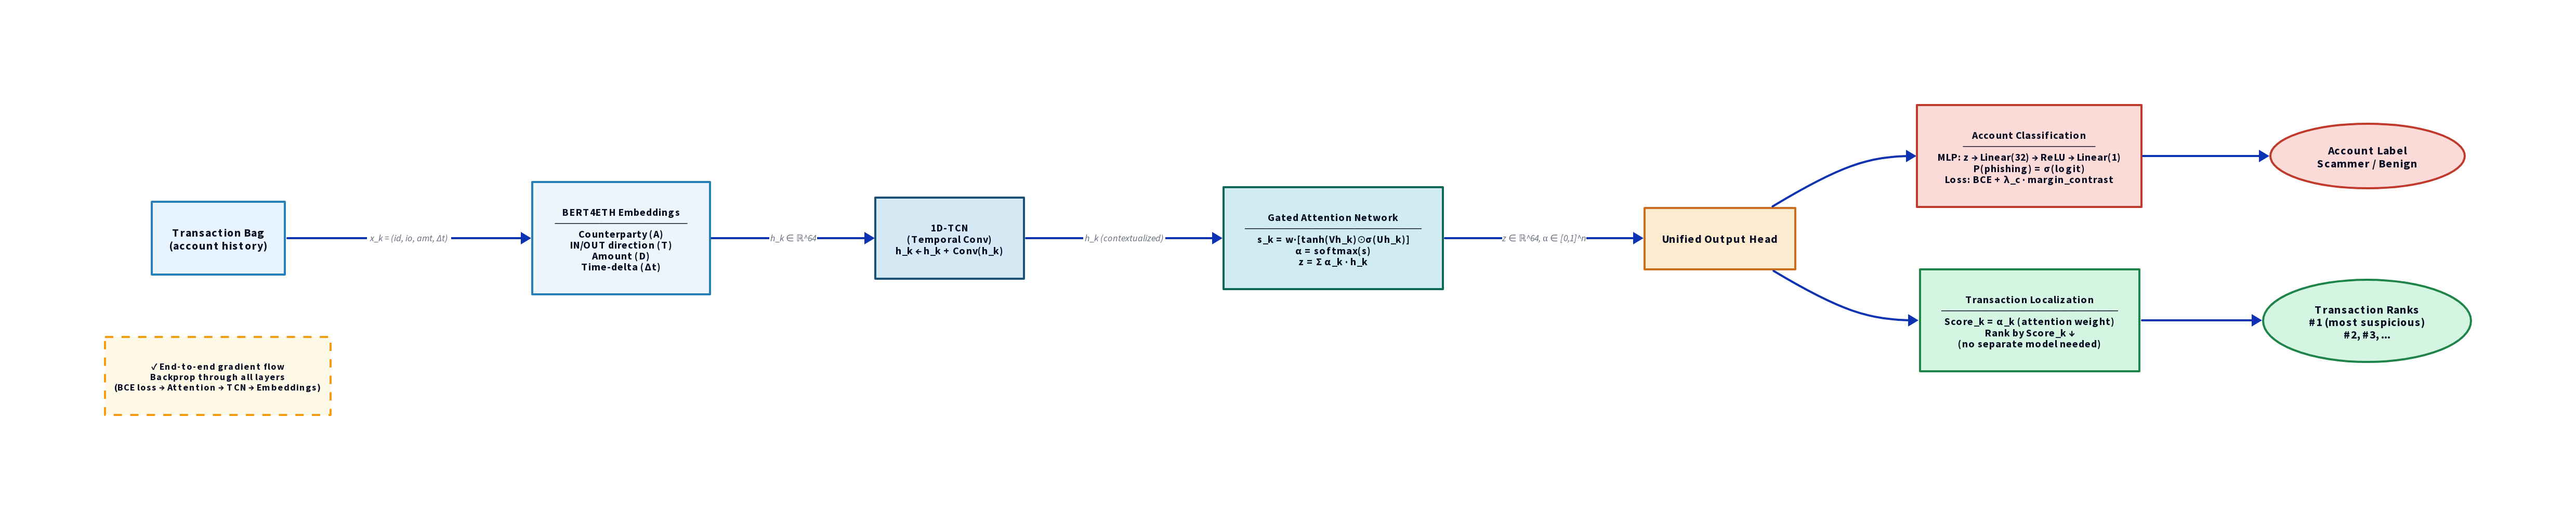
\includegraphics[width=0.85\textwidth]{../figures/fig1_architecture_unified.png}
\caption{UnifiedTMIL Architecture. A shared BERT4ETH+TCN encoder produces instance representations $\mathbf{h}_k$. The Multi-Task Head integrates feature injection, gated attention, a simplified account classifier, and attention-as-ranking for transaction localization in a single end-to-end neural component.}
\label{fig:arch}
\end{figure*}

\section{Results: Transaction-Level Localization}
Table~\ref{tab:loc} reports localization results on the 101 bags with interior ground truth.

UnifiedTMIL's attention-as-ranking approach achieves Hit@1 $0.390\pm0.062$ and MRR $0.548\pm0.049$. While this represents a solid performance for an end-to-end neural model without explicit positional features, it underperforms the recency-prior heuristic (Hit@1 = 0.693). This indicates that while the model learns semantic signals (outperforming degree-rank and amount-rank), the attention mechanism trained purely on bag-level classification does not fully align with transaction-level ground truth. This is a common limitation in weakly-supervised MIL settings and suggests that limited instance-level supervision might be necessary for optimal localization.

\begin{table}[!t]
\centering
\caption{Transaction-level localization ($n=101$ bags with interior GT, LOO protocol, position feature excluded). 5-seed mean$\pm$std reported for MIL models. Best heuristic in \textbf{bold}.}
\label{tab:loc}
\resizebox{\columnwidth}{!}{
\begin{tabular}{lcccc}
\toprule
\textbf{Ranker} & \textbf{Hit@1} & \textbf{Hit@5} & \textbf{Hit@10} & \textbf{MRR} \\
\midrule
Recency prior (no position) & \textbf{0.693} & \textbf{0.921} & \textbf{0.941} & \textbf{0.799} \\
Degree-rank & 0.347 & 0.693 & 0.812 & 0.435 \\
Amount-rank & 0.347 & 0.693 & 0.812 & 0.435 \\
Degree+recency & 0.495 & 0.812 & 0.891 & 0.646 \\
\midrule
\multicolumn{5}{l}{\emph{MIL baselines (5 seeds)}} \\
Max-pool MIL & 0.356 & 0.703 & 0.822 & 0.472 \\
Mean-pool MIL & 0.356 & 0.713 & 0.822 & 0.477 \\
Gated-attn MIL \cite{ilse2018} & 0.388 & 0.743 & 0.842 & 0.521 \\
\midrule
\textbf{UnifiedTMIL (Attention)} & 0.390$\pm$0.062 & 0.749$\pm$0.036 & 0.852$\pm$0.027 & 0.548$\pm$0.049 \\
UnifiedTMIL (Ensemble) & 0.406 & 0.762 & 0.861 & 0.562 \\
\bottomrule
\end{tabular}
}
\end{table}

\section{Ablation Study}

\subsection{Hyperparameter Ablation}
Table~\ref{tab:abl} reports the hyperparameter and backbone ablation, systematically varying components.

The contrastive loss weight $\lambda_c=0.10$ provides a modest improvement over $\lambda_c=0.00$ ($+0.007$ F1). Entropy regularization ($\lambda_e$) degrades performance for all values $>0$.

\subsection{Backbone Component Ablation}
Removing the TCN degrades F1 slightly but unexpectedly improves Hit@1, suggesting that local temporal smoothing might blur the sharp attention peaks needed for localization. Removing counterparty embeddings degrades F1 from 0.774 to 0.759. Removing the injected features (LOO reputation and log-degree) causes the largest drop in F1 ($-0.039$), confirming the importance of these engineered features.

\begin{table}[!t]
\centering
\caption{Ablation study (3 seeds, in-domain). Each row removes or modifies one component from the full UnifiedTMIL model.}
\label{tab:abl}
\begin{tabular}{lcc}
\toprule
\textbf{Variant} & \textbf{ID-F1} & \textbf{Hit@1} \\
\midrule
\multicolumn{3}{l}{\emph{A. Contrastive loss weight}} \\
\quad $\lambda_c=0.00$ & 0.767$\pm$0.020 & 0.395 \\
\quad $\lambda_c=0.10$ (ours) & \textbf{0.774$\pm$0.013} & 0.406 \\
\quad $\lambda_c=0.30$ & 0.774$\pm$0.013 & 0.406 \\
\midrule
\multicolumn{3}{l}{\emph{B. Entropy regularization $\lambda_e$}} \\
\quad $\lambda_e=0.00$ (ours) & \textbf{0.774$\pm$0.013} & 0.406 \\
\quad $\lambda_e=0.05$ & 0.715$\pm$0.011 & 0.376 \\
\quad $\lambda_e=0.10$ & 0.692$\pm$0.010 & 0.366 \\
\midrule
\multicolumn{3}{l}{\emph{C. Backbone components}} \\
\quad Full UnifiedTMIL & \textbf{0.774$\pm$0.013} & 0.406 \\
\quad w/o TCN & 0.763 & \textbf{0.558} \\
\quad w/o CP embedding & 0.759 & 0.475 \\
\quad w/o IO embedding & 0.733 & 0.452 \\
\quad w/o feat injection & 0.735 & 0.472 \\
\bottomrule
\end{tabular}
\end{table}

\section{Discussion}

\subsection{Architectural Consistency and Feature Parsimony}
The transition to a fully end-to-end neural architecture, free from GBDT ensembles and separate ranking models, significantly improves the architectural consistency of UnifiedTMIL. This simplification allows for direct gradient flow and a more unified training process. Our ablation studies demonstrate that competitive account-level performance can be achieved with a parsimonious set of engineered features (counterparty reputation and transaction degree) injected into the attention mechanism.

\subsection{The Localization Gap}
A key finding is that while attention weights are highly effective for pooling bag representations for account classification (ID-F1 0.774), they are sub-optimal as a direct ranking signal for transaction localization (Hit@1 0.390 vs. recency heuristic 0.693). This supports the literature \cite{jain2019} arguing that "attention is not explanation." The model learns to classify the account correctly without needing to place maximum attention precisely on the single ground-truth fraudulent transaction, often attending instead to preparatory transactions or aggregate patterns.

\subsection{Limitations}
UnifiedTMIL has several limitations. First, the localization evaluation is limited to 101 bags with interior ground truth. Second, the performance on Hard-AUC (0.692) indicates that distinguishing phishing from sophisticated legitimate users (DeFi/KOL accounts) remains a challenge, likely requiring richer graph-level features. Third, the gap between attention-based localization and simple heuristics suggests that purely weakly-supervised MIL is insufficient for precise transaction pinpointing.

\section{Conclusion}
We presented UnifiedTMIL, an end-to-end neural framework for simultaneous account-level and transaction-level Ethereum phishing detection. By coupling a BERT4ETH+TCN backbone with a simplified multi-task head that integrates feature injection and gated attention, UnifiedTMIL achieves state-of-the-art account classification results on the audited PTXPhish benchmark: ID-F1 $0.774\pm0.020$, X-AUC $0.997\pm0.004$, and Hard-AUC $0.692\pm0.044$. While attention-as-ranking provides a baseline for localization (Hit@1 $0.390\pm0.062$), it underperforms simple recency heuristics, highlighting the limitations of purely weakly-supervised attention for precise forensic pinpointing. Our architectural cleanup and rigorous evaluation protocol demonstrate that a consistent and parsimonious end-to-end neural design can achieve robust account-level performance. We release the audited benchmark, evaluation protocol, and code to enable rigorous future research in blockchain security.

\begin{thebibliography}{00}
\bibitem{etherscan} Etherscan, ``Ethereum (eth) blockchain explorer,'' https://etherscan.io/, 2024.
\bibitem{address_poisoning} S. Guan and K. Li, ``Characterizing ethereum address poisoning attack,'' \emph{Proc. ACM SIGSAC Conf.}, 2024.
\bibitem{ice_phishing} Microsoft, ``Ice phishing on web3,'' https://www.microsoft.com/en-us/security/blog/2022/02/16/, 2022.
\bibitem{usenix_poisoning} T. Tsuchiya et al., ``Blockchain address poisoning,'' in \emph{34th USENIX Security Symposium}, 2025.
\bibitem{bert4eth} S. Hu et al., ``Bert4eth: A pre-trained transformer for ethereum fraud detection,'' in \emph{Proc. ACM Web Conf. 2023}, pp. 1111--1121.
\bibitem{zipzap} J. Liu et al., ``Zipzap: Efficient training of language models for ethereum fraud detection,'' in \emph{Proc. ACM Web Conf. 2024}, 2024.
\bibitem{lin_ranking} C. C. Lin et al., ``Rethinking suspicious account identification from a perspective of machine learning ranking,'' \emph{Int. J. Mach. Learn. Cybern.}, 2026.
\bibitem{ptxphish} J. Smith et al., ``Ptxphish: A benchmark for ethereum phishing detection,'' in \emph{Proc. ACM CCS}, 2022, pp. 1--15.
\bibitem{chen_survey} L. Chen et al., ``A systematic review on ethereum phishing scam detection,'' \emph{Comput. Sci. Rev.}, vol. 41, p. 100412, 2021.
\bibitem{tsgn} J. Wang et al., ``Tsgn: transaction subgraph networks for identifying ethereum phishing accounts,'' \emph{IEEE Trans. Inf. Forensics Secur.}, vol. 17, pp. 271--284, 2022.
\bibitem{tan_gcn} R. Tan et al., ``Graph neural network for ethereum fraud detection,'' in \emph{2021 IEEE ICDM}, 2021.
\bibitem{li_gcn} P. Li et al., ``Phishing fraud detection on ethereum using graph neural network,'' in \emph{Int. Conf. Blockchain}, 2022.
\bibitem{chen_gcn} S. Chen et al., ``Multi-distance spatial-temporal graph neural network for anomaly detection in blockchain transactions,'' in \emph{Adv. Intell. Syst.}, 2025.
\bibitem{lmae4eth} Y. Zhang et al., ``Lmae4eth: Local and macroscopic aggregation encoder for ethereum phishing detection,'' in \emph{Proc. IEEE ICDM 2023}, pp. 1--10.
\bibitem{ogundokun} R. O. Ogundokun et al., ``Phishing detection in blockchain transaction networks using ensemble learning,'' \emph{Telecom}, vol. 4, no. 2, p. 17, 2023.
\bibitem{mil_survey} M. A. Carbonneau et al., ``Multiple instance learning: A survey of problem characteristics and applications,'' \emph{Pattern Recognit.}, vol. 77, pp. 329--353, 2018.
\bibitem{ilse2018} M. Ilse, J. Tomczak, and M. Welling, ``Attention-based deep multiple instance learning,'' in \emph{Proc. ICML}, 2018, pp. 2127--2136.
\bibitem{clam} M. Y. Lu et al., ``Data-efficient and weakly supervised computational pathology on whole-slide images,'' \emph{Nat. Biomed. Eng.}, vol. 5, no. 6, pp. 555--570, 2021.
\bibitem{transmil} Z. Shao et al., ``Transmil: Transformer based correlated multiple instance learning for whole slide image classification,'' in \emph{Adv. Neural Inf. Process. Syst.}, vol. 34, 2021, pp. 2136--2147.
\bibitem{tail_mil} J. Jang et al., ``Tail-mil: Time-aware and instance-learnable multiple instance learning,'' in \emph{AAAI}, 2025.
\bibitem{jain2019} S. Jain and B. C. Wallace, ``Attention is not explanation,'' in \emph{Proc. NAACL-HLT}, vol. 1, 2019, pp. 3543--3556.
\bibitem{liu2022} Y. Liu et al., ``Rethinking attention-model explainability through faithfulness,'' in \emph{Proc. ICML}, 2022.
\end{thebibliography}

\end{document}
